\documentclass[../../main.tex]{subfiles}
\begin{document}
%
    In this chapter we aim at combining what has been learnt throughout the previous chapters, namely, to go from two distinct models to one that is capable of representing the cross-linked nature of these bio-polymers. We will focus on two distinct setups, resulting from the different placement of cross-linkers across the polymer chain.
    
    Consider a five-monomer chain where, as in \cref{ch: Gaussian Chain}, the monomers interact via an harmonic potential (\cref{eq: Gaussian Chain - Harmonic Spring Potential}). The different chains will only interact through their cross-linkers, allowing for the overlap of all other monomers. The potential, $U_{\beta}$, introduced in \cref{ch: Particle-Particle Aggregation} (see \cref{eq: L-J - New Potential}) will be used to model such cross-link interactions.
    
    We first look at the addition of a cross-linker monomer in the middle of the chain. Note that, by using \cref{eq: Gaussian Chain - Harmonic Spring Potential}, we have that all the particles of a chain will experience a pull towards the centre, and the chain will act as one big colloidal particle, in a system which will, undoubtedly, resemble the one presented in \cref{ch: Particle-Particle Aggregation}.
    %
        \begin{figure}[h]
            \centering
            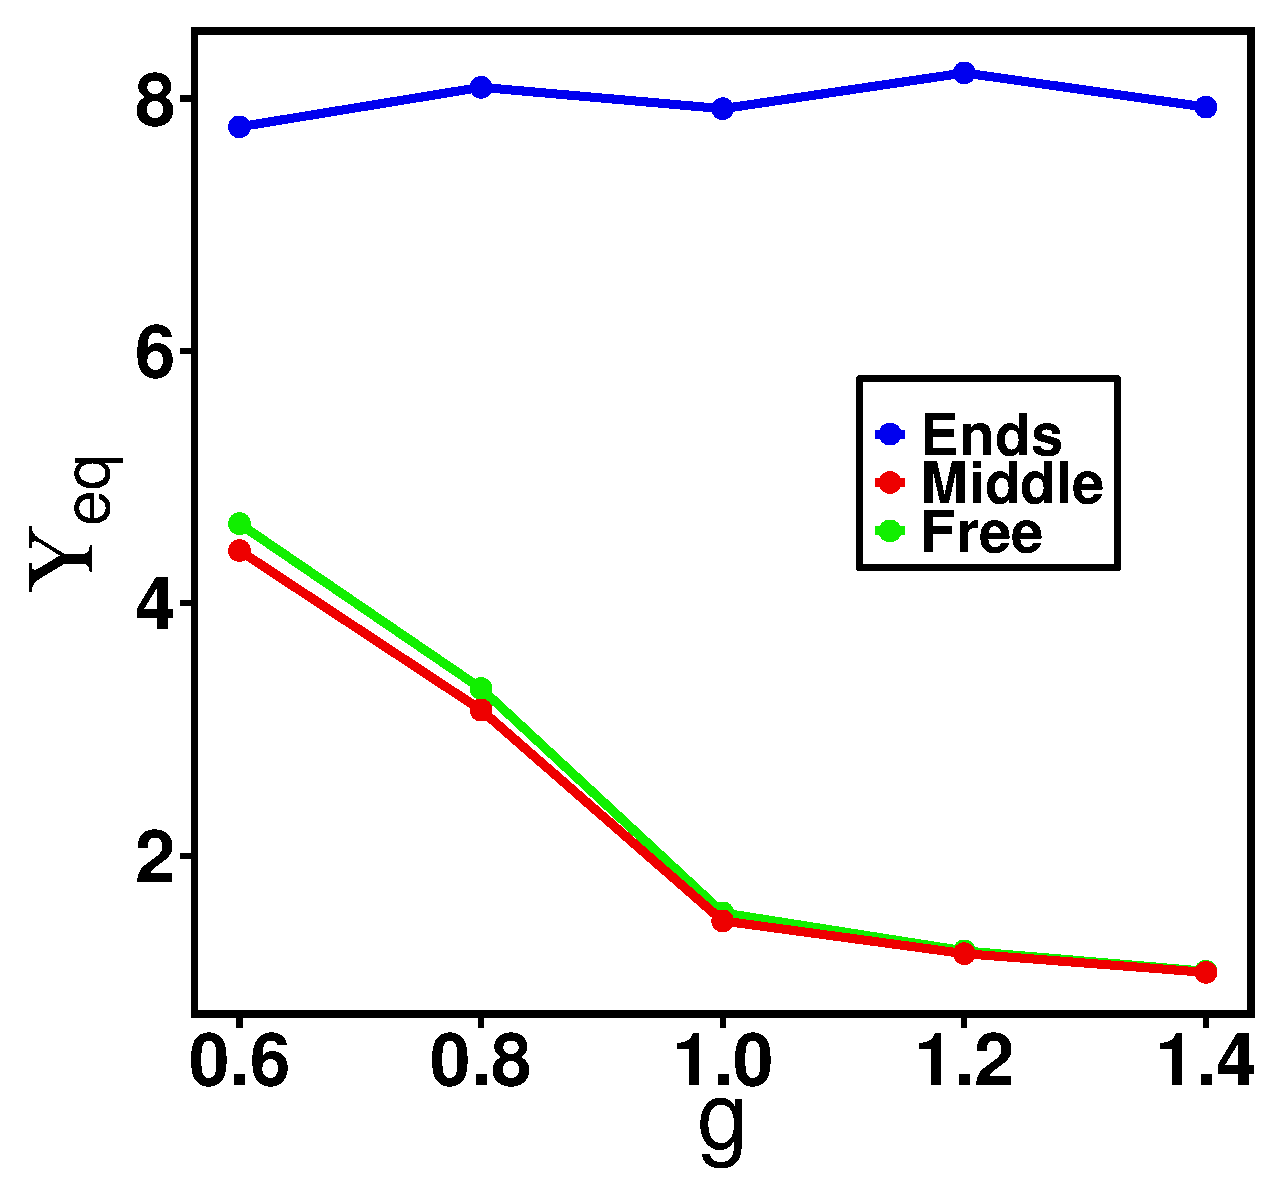
\includegraphics[scale=0.4]{Figures/no_repel.eps}
            \caption{Comparison between three models: free particle, five monomer chain with one cross-linker placed at the centre and five monomer chain with two cross-linker placed at ends. The first two cases experience roughly the same behaviour since, in the limit where $\kappa \rightarrow \infty$, they should be equal. By placing the cross-linkers at the extremities of the chain, we appear to have created a more stable network, where $\Upsilon_{eq}$ remains the same independently of $g$. Parameters used: $\kappa_s = 5$, $\upsilon = 1$, $\epsilon = 1$, $h = 0.8$, $w = 0.15$, $r_b = 1.52$, $\rho = 2/15$.}
            \label{fig: no repel - comparison}
        \end{figure}
        
    Placing the cross-linkers at the ends of the chain might make us expect that the different chains would pull one another, which in turn would lead to their extension. What actually happens is that the different chains get pulled together to form larger clusters. More often then not, when two cross-linkable monomers form a bond, their chain counterparts rapidly comply to completely connect the two chains. Setting the density of cross-linkers constant between the two models, we now expect that the number of bonds per cross-link to be greater in the second since it is easier to ``pull" chains together. This is indeed what happens. In \cref{fig: no repel - comparison}, we see that the system with the cross-linker monomer in the middle of the chain behaves very similarly to the free colloidal particle model. When comparing the two, $\Upsilon_{eq}$ is lower when $g<1$ for the case of the polymer chain. Moreover, the time it takes for the system to reach a stationary state (not shown here) is longer. The results might be explained by the higher drag which is produced by the rest of the chain, hindering the movement of the cross-linker and consequently its ability to form bonds. What is surprising is the stability of $\Upsilon_{eq}$ to the change of $g$ in the case where the cross-linkers are place at the ends of the chain. The behaviour can be explained if we consider the structures formed that were previously discussed. By having a second cross-linker connecting the two different chains, it becomes harder for them to detach once the bonds are formed, for even if one breaks, the chain will still be in the surrounding perimeter and it can reattach itself. What will happen is that the time for the system to relax from a disordered state might be different but, at least for the systems tested, they will reach a similar relaxed state.
\begin{comment}
    It appears that $\Upsilon_{eq}$ doesn't rise as fast for low temperatures, a possible result of a heavier ``particle" where the cross-linker gets pulled by the other monomers in its chain, hindering the formation of bonds. 
\end{comment}    
    
    By choosing to ignore interactions between monomers of different chains, we have constructed a rather unrealistic representation of polymer chains in solution. These steric effects are very common and so, to complement the previous model, a repulsive force arising from all interactions between monomers of different chains is added. We chose the L-J potential (\cref{eq: L-J - Lennard-Jones Potential}) for this effect, since, by truncating it at $r_{min}$, we are able to consider only its repulsive part. Adding to this fact, the L-J potential had already been used throughout this work making its implementation in the model straightforward.
    
    From here, we focus on two different cases: with the cross-linker placed in the middle, it would make sense that, as two chains approach, their ends would bend backwards, allowing for the two cross-link capable monomers to form a bond, connecting their respective chains; in the case of the two cross-linker monomers placed at the ends of the chain, we would expect that, either the two chains in question would extend, allowing for the connection of all cross-linkers or, it would foster connections between more than two chains, since one end of each chain would be able to connect and then, the repulsion between non cross-link capable monomers from both chains, would drive the other end away, making it free to form other connections. 
        \begin{figure}[h]
            \centering
            \begin{subfigure}[b]{0.47\textwidth}
                \centering
                \includegraphics[width=\textwidth]{Figures/middle_ovito.png}
                \caption{}
                \label{fig: ovito - repel - middle}
            \end{subfigure}
            \hfill
            \begin{subfigure}[b]{0.47\textwidth}
                \centering
                \includegraphics[width=\textwidth]{Figures/ends_ovito.png}
                \caption{}
                \label{fig: ovito - repel - ext}
            \end{subfigure}
            \hspace*{\fill}
            \begin{minipage}[t]{\textwidth}
                \centering
                \includegraphics[scale=0.07]{Figures/legenda2.png}
            \end{minipage}
            \caption{Final iteration of the numerical simulation based on the model that considers repulsion between monomers of different chains. In \cref{fig: ovito - repel - middle}, cross-linkers are placed in the middle of the chain. We note that only a small portion of chains are able to form a link. This becomes all the more evident when we look at \cref{fig: ovito - repel - ext}, where the cross-linkers were placed at the ends of the chain. In addition to the higher number of chains interacting and bonds being formed, we observe a new behaviour, with the overlapping of cross-linkers and the chain repelling core pointing outwards. Parameters used: $\kappa_s = 5$, $\upsilon = 1$, $\epsilon = 1$, $h = 0.8$, $w = 0.15$, $r_b = 1.52$, $\rho = 2/15$.}
            \label{fig: ovito - repel}
        \end{figure}   
    
    This does not appear to happen. In \cref{fig: ovito - repel} we have the final state of simulations for both cases under the same conditions of \cref{fig: no repel - comparison}. Even without a plot quantifying $\Upsilon_{eq}$, a qualitatively analysis of \cref{fig: ovito - repel - middle} shows very few bonds formed. This result is explained by the gathering of monomers around the centre of the chain, promoted by the spring potential introduced in \cref{ch: Gaussian Chain}, whose equilibrium position is zero. Repulsion will now dominate, making the cross-link attractive potential negligible and keeping the two monomers from establishing a bond. We still notice the expected behaviour but at a much smaller scale. In \cref{fig: ovito - repel - ext}, we notice a strange behaviour. The two cross-linkers from each polymer chain overlap each other. What appears a similar structure to that formed in \cref{fig: ovito - repel - middle}, is in fact a chain connected by its two end points, with its core extended outwards. This doubles the attractive potential while at the same time keeps the repelling monomers at bay, allowing for more bonds to be formed.
    
        \begin{figure}[h]
            \centering
            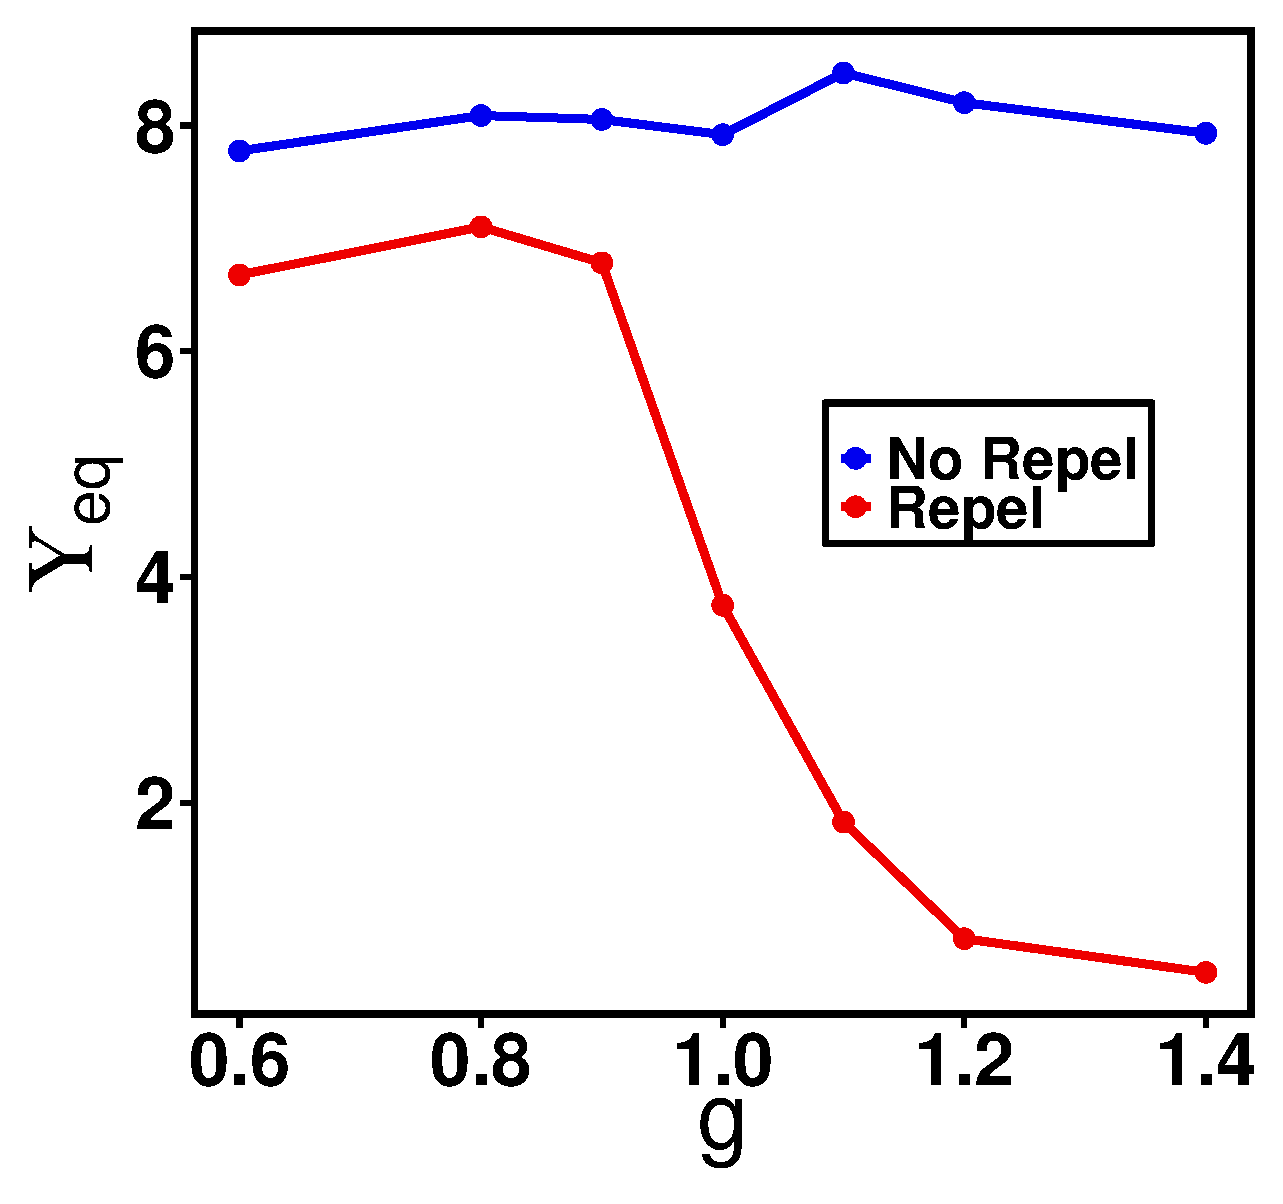
\includegraphics[scale=0.40]{Figures/repel_vs_no.eps}
            \caption{Comparison between two different models: with repulsive interactions between monomers of different chains and without; cross-linkers are placed at the ends of the chains in both cases. We note again a transition between two regimes, occurring faster and at a higher $g$ than the one presented in \cref{fig: no repel - comparison} for the free particle/middle placement of the cross-linker. Parameters used: $\kappa_s = 5$, $\upsilon = 1$, $\epsilon = 1$, $h = 0.8$, $w = 0.15$, $r_b = 1.52$, $\rho = 2/15$.}
            \label{fig: no repel vs repel}
        \end{figure}
    
    In \cref{fig: no repel vs repel}, we draw a comparison between the two models with cross-linkers placed at the ends of the chain. The addition of repulsion between chains seems to have brought back a transition between a regime that favours bond formation and another that does not. As the temperature increases, so do random motions, making it harder for the chains to arrange, and maintain, the repelling core away from the cross-linkers attractive potential.
    
    We showed that the placement of the cross-linker in the chain has a direct influence on the size and stability of the network formed. With the addition of repulsion between different chains, we can still recover a regime with a high number of bonds formed, however, under those conditions, instead of the overarching network first envisioned, we observe multiple isolated clusters.

  
%
\end{document}